Asumiendo que debido a igual proceso de fabricación, se cumple $V_{THn} = -V_{THp}$, se puede deducir a partir de los calculos de las resistencias de salida de las etapas de las compuertas.

\subsection{Compuerta NOR}
\begin{equation}
    \frac{\beta_n}{\beta_p} = \frac{k_{p_n}\frac{W_n}{2\cdot L_n}}{k_{p_p}\frac{W_p}{L_p}} = \frac{1}{2}
\end{equation}

Entonces para $W_n = 2 \mu m$, la condición impone $W_p = 12 \mu m$.

Esto produce la siguiente respuesta $V_{(V_{i})}$:

\begin{figure}[H]
    \centering
    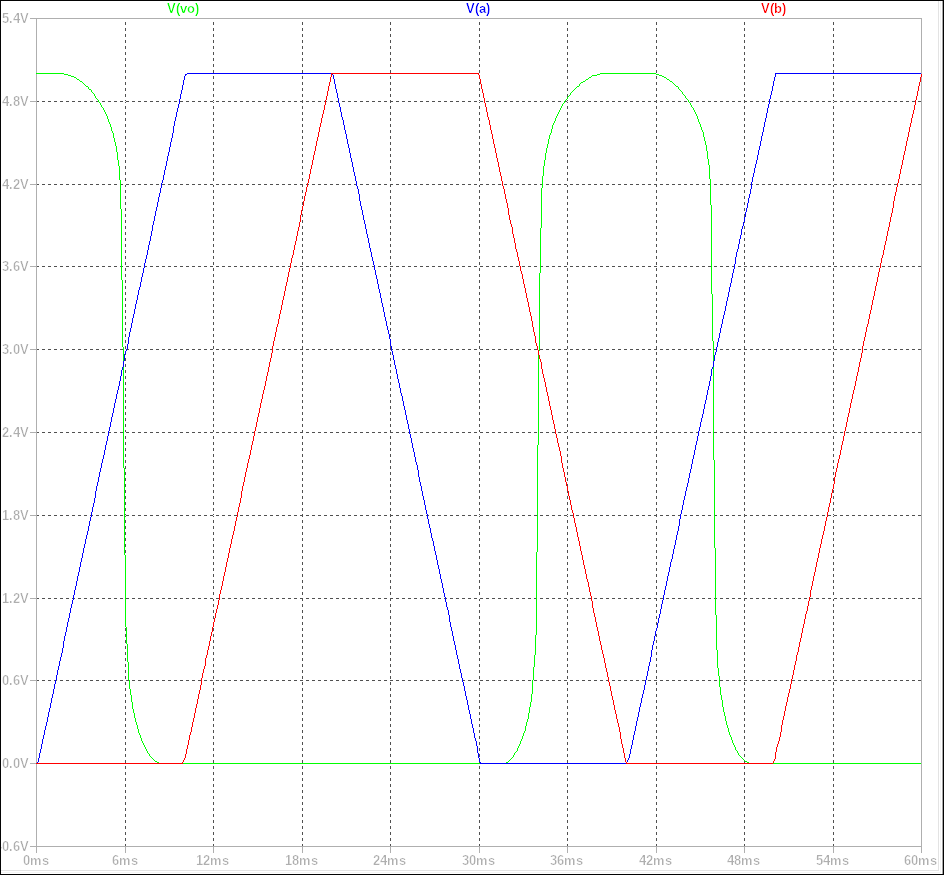
\includegraphics[width=0.8\textwidth]{Imagenes/NOR12u.png}
    \caption{Respuesta Celda NOR con $W_p = 12\mu m$}
    \label{fig:norChoto}
\end{figure}
Como se puede observar en la simulación este resultado implica que $V_{sp} \neq \frac{V_{DD}}{2}$.

Para esto se necesita $W_p \approx 6 \mu m$.
\begin{figure}[H]
    \centering
    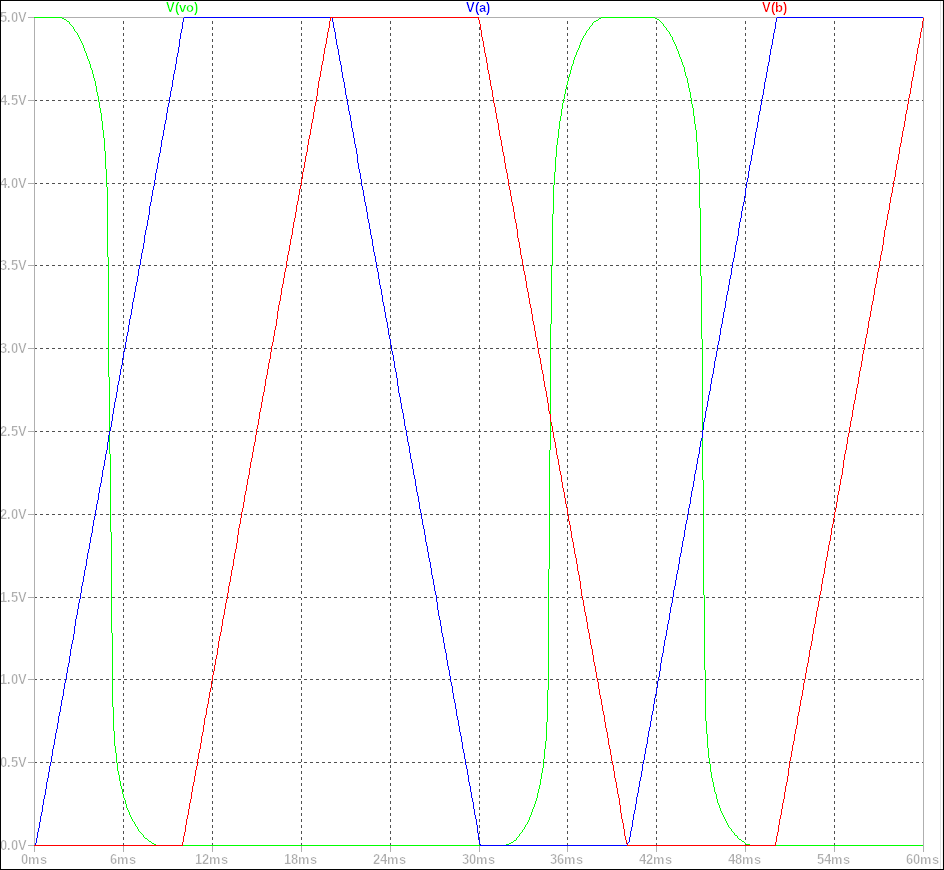
\includegraphics[width=0.8\textwidth]{Imagenes/NOR6u.png}
    \caption{Respuesta Celda NOR con $W_p \approx 6\mu m$}
    \label{fig:norBueno}
\end{figure}

\subsection{Compuerta NAND}
\begin{equation}
    \frac{\beta_n}{\beta_p} = \frac{k_{p_n}\frac{W_n}{L_n}}{k_{p_p}\frac{W_p}{2\cdot L_p}} = 2
\end{equation}

Entonces, con $W_n = 2\mu m$, la condición impone $W_p = 3 \mu m$.

Esto produce la siguiente respuesta $V_{(V_{i})}$:

\begin{figure}[H]
    \centering
    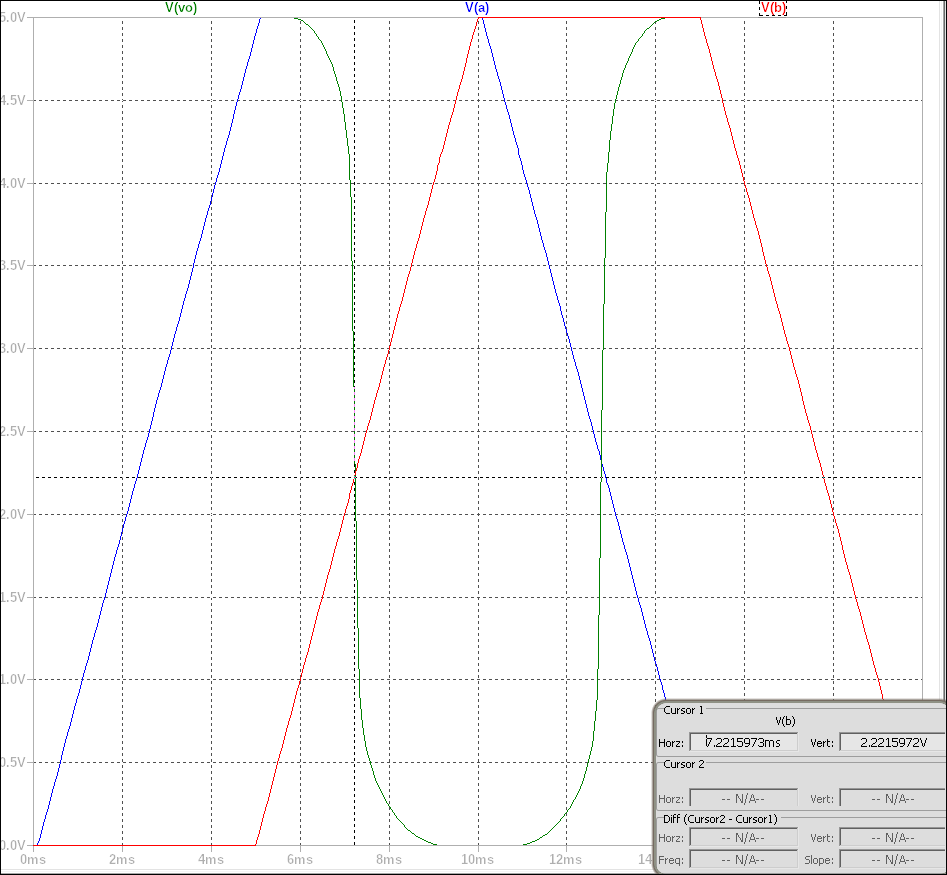
\includegraphics[width=0.8\textwidth]{Imagenes/NAND3u.png}
    \caption{Respuesta Celda NAND con $W_p = 3\mu m$}
    \label{fig:nandChoto}
\end{figure}

Pero en la simulación se encontró que se necesita $W_p = 4.8 \mu m$:

\begin{figure}[H]
    \centering
    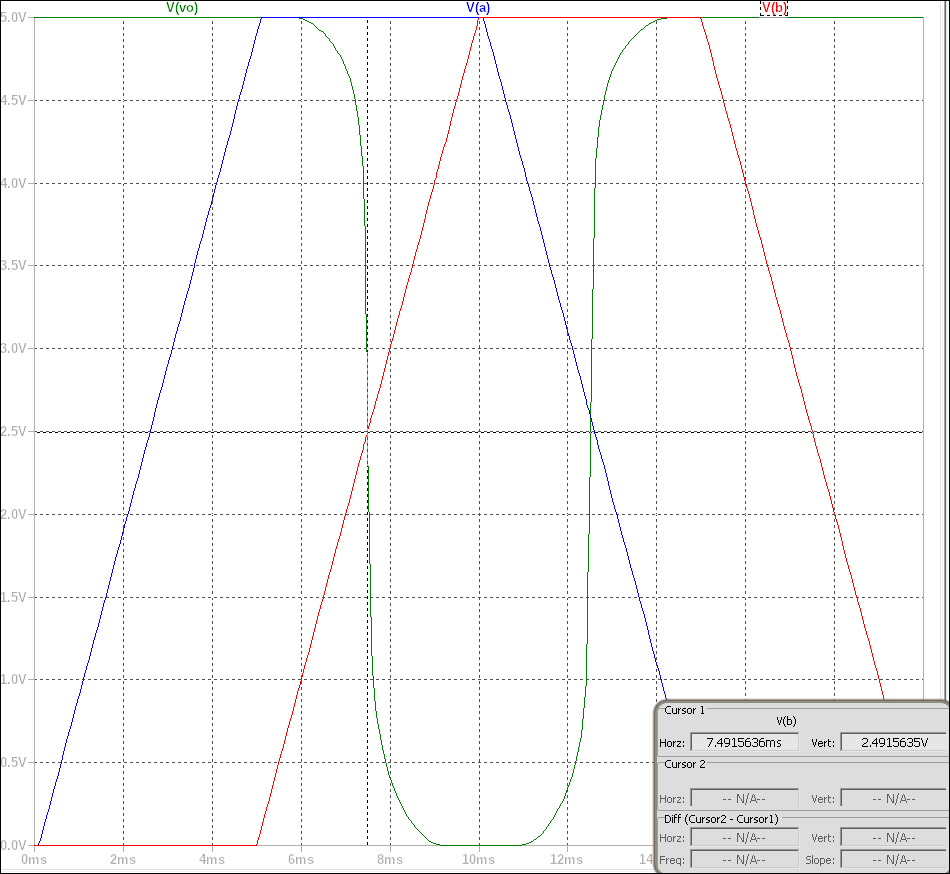
\includegraphics[width=0.8\textwidth]{Imagenes/NAND4u8.png}
    \caption{Respuesta Celda NAND con $W_p = 4.8\mu m$}
    \label{fig:nandBueno}
\end{figure}

